\documentclass[twocolumn,a4j]{jsarticle}
\setlength{\topmargin}{-20.4cm}
\setlength{\oddsidemargin}{-10.4mm}
\setlength{\evensidemargin}{-10.4mm}
\setlength{\textwidth}{18cm}
\setlength{\textheight}{26cm}

\usepackage[top=15truemm,bottom=20truemm,left=20truemm,right=20truemm]{geometry}
\usepackage[latin1]{inputenc}
\usepackage{amsmath}
\usepackage{amsfonts}
\usepackage{amssymb}
\usepackage[dvipdfmx]{graphicx}
\usepackage[hang,small,bf]{caption}
\usepackage[subrefformat=parens]{subcaption}
\usepackage[dvipdfmx]{color}
\usepackage{listings}
\usepackage{listings,jvlisting}
\usepackage{geometry}
\usepackage{framed}
\usepackage{color}
\usepackage[dvipdfmx]{hyperref}
\usepackage{ascmac}
\usepackage{enumerate}
\usepackage{tabularx}
\usepackage{cancel}
\usepackage{scalefnt}
\usepackage{overcite}
\usepackage{otf}
\usepackage{multicol}
\usepackage[geometry]{ifsym}

\renewcommand{\figurename}{Fig.}
\renewcommand{\tablename}{Table }

\hypersetup{%
    hidelinks %リンクの色消し
}

\lstset{
basicstyle={\ttfamily},
identifierstyle={\small},
commentstyle={\smallitshape},
keywordstyle={\small\bfseries},
ndkeywordstyle={\small},
stringstyle={\small\ttfamily},
frame={tb},
breaklines=true,
columns=[l]{fullflexible},
xrightmargin=0zw,
xleftmargin=3zw,
numberstyle={\scriptsize},
stepnumber=1,
numbersep=1zw,
lineskip=-0.5ex
}

% キャプション後ろのダブルコロンを消す
\makeatletter
\long\def\@makecaption#1#2{%
  \vskip\abovecaptionskip
  \iftdir\sbox\@tempboxa{#1\hskip1zw#2}%
    \else\sbox\@tempboxa{#1 #2}%
  \fi
  \ifdim \wd\@tempboxa >\hsize
    \iftdir #1\hskip1zw#2\relax\par
      \else #1 #2\relax\par\fi
  \else
    \global \@minipagefalse
    \hbox to\hsize{\hfil\box\@tempboxa\hfil}%
  \fi
  \vskip\belowcaptionskip}
\makeatother


\makeatletter
\def\@maketitle
{
\begin{center}
{\LARGE \@title \par}
\end{center}
\begin{flushright}
{\large \@date}\\
{\large 京都工芸繊維大学 大学院 機械設計学専攻 計測システム工学研究室}\\
{\large M2 \@author}
\end{flushright}
\par\vskip 1.5em
}
\makeatother

\author{来代 勝胤 / KITADAI Masatsugu}
\title{令和5年度 9月度 共同研究報告書}
\date{2023/09/29}

\begin{document}
\columnseprule=0.1mm
\maketitle

\section*{報告内容}
\begin{enumerate}[1.]
	\item ISTP-33 について
	\item 解析手順の再構成
	\item 10月の予定
\end{enumerate}

\section*{進捗報告}
今月は,9/24 - /27 まで ISTP-33 に参加し
研究発表を行った.
また,先月に引き続き,二次流れ解析プログラムの性能向上を目的に
アルゴリズムの見直しや処理の検討を行っている.

\section{ISTP-33 について}
\begin{table}[hbtp]
	\label{table:data_type}
	\begin{tabular*}{9cm}{ c | c }
		\hline
		\textgt{題目} & \begin{tabular}{c} Performance Evaluation of PIV Measurement \\ of Secondary Flow using Multi-Color LLS \end{tabular}        \\ \hline
		\textgt{内容} & \begin{tabular}{c} 数値シミュレーションを用いた\\計測手法の精度評価の結果について \end{tabular}        \\ \hline
		\textgt{日時} & 2023/9/24 - 9/27                 \\ \hline
		\textgt{会場} & 熊本県 熊本市中央区 熊本城ホール\\ \hline
	\end{tabular*}
\end{table}

\section{解析手順の再構成}
これまで検討を行ってきた解析の一連の流れとアルゴリズムについて,
性能向上と解析手順の明確化のため見直しを行っている.

\begin{enumerate}[(1)]
	\item [] \textgt{[ 全体の流れ ]}
	\item 校正ブロックの校正点特定と補正関数の取得 (完了)
	\item 背景処理・粒子位置特定等の前処理 (完了)
	\item 粒子追跡 (検討中)
	\item ベクトルの再配置・誤ベクトル除去等の後処理 (検討中)
\end{enumerate}

\section{(3) 粒子追跡:同一粒子の判別}
レーザーシートを通過する粒子が複数枚の画像内に同一の粒子像が現れ,
流れ場の解析時に問題となる場合がある.
また,主流方向速度が局所的に変動する場合,粒子の追跡が困難となるため
おおよその粒子の持つ主流方向速度の情報を知る必要がある.
そこで,今回は粒子像を画像の時刻経過に沿ってクラスタリングを行い,
その結果から粒子位置の特定や粒子の持つ速度情報の取得を試みた.

\begin{figure}[htbp]
	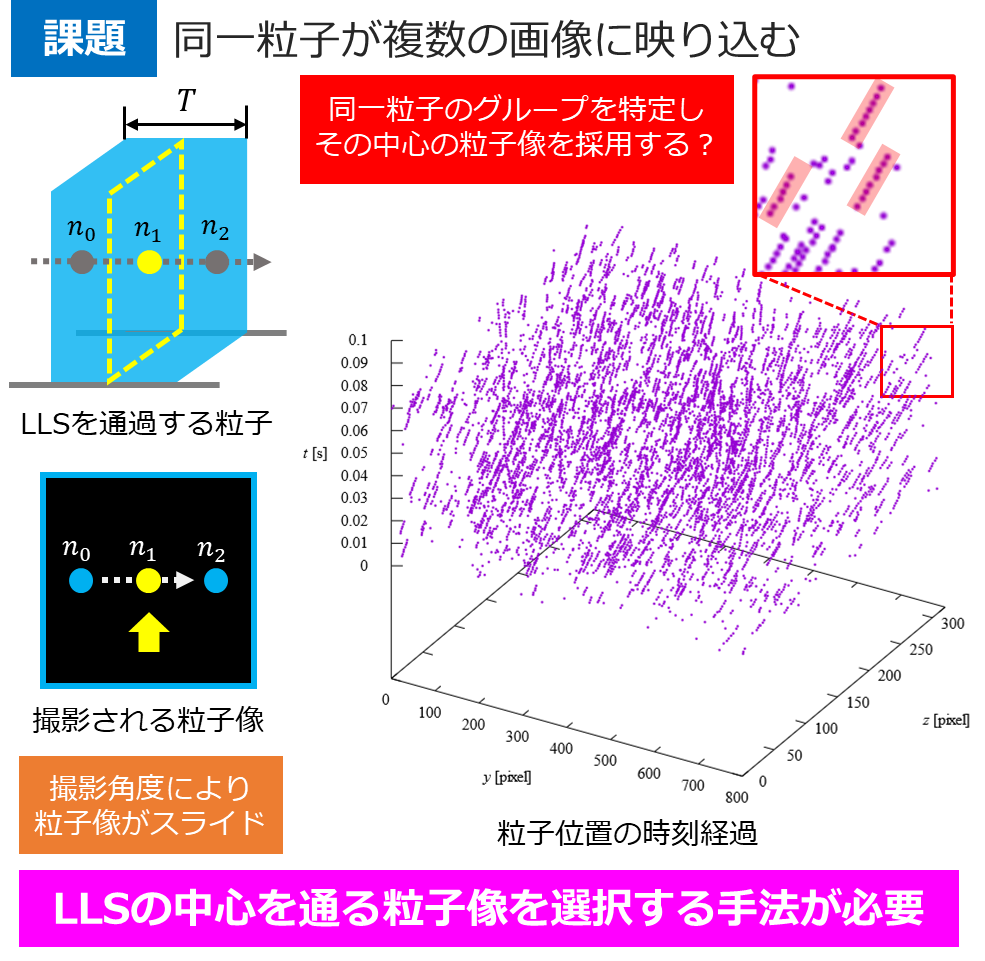
\includegraphics[keepaspectratio, width=82mm]{../images/challenge.png}
\end{figure}

\subsection{粒子像のクラスタリング}
\begin{figure}[htbp]
	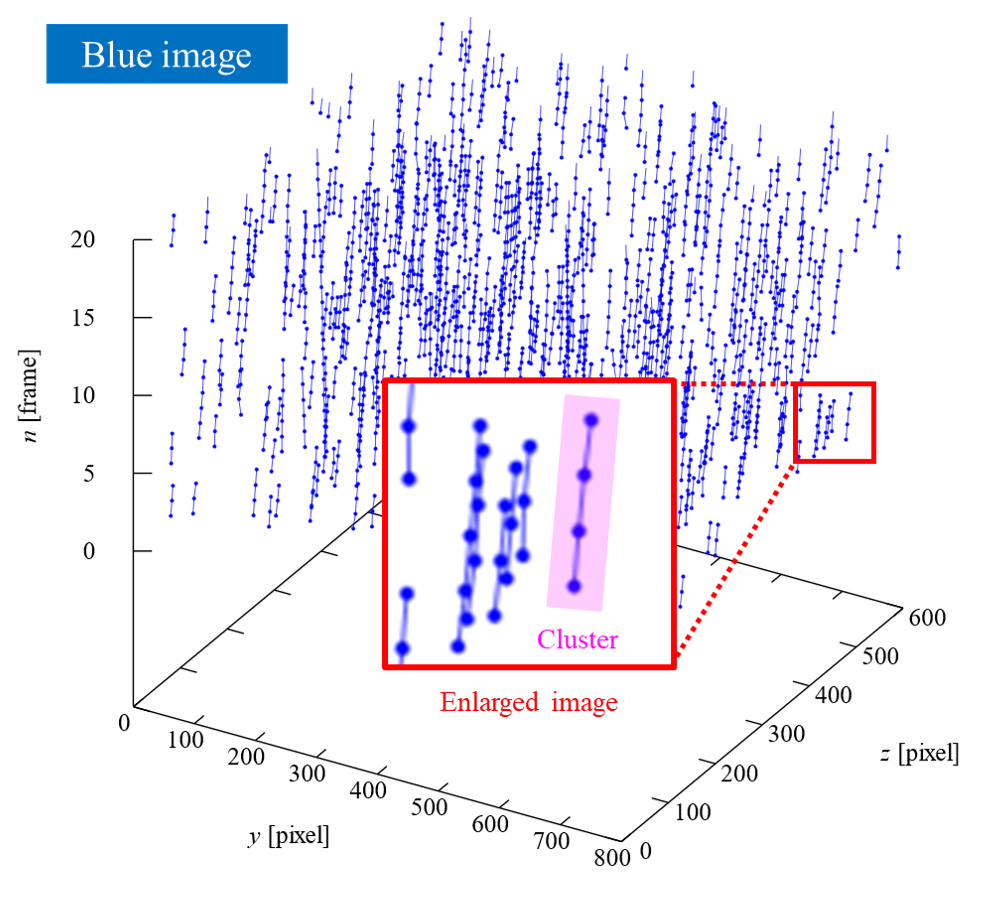
\includegraphics[keepaspectratio, width=82mm]{../images/cluster_for_b.png}
\end{figure}


\subsection{粒子像の位置決定}
\subsection{クラスタのマッチング}

\section{(4) ベクトルの再配置・誤ベクトル除去等の後処理}
\section{ガウシアンフィルタによる再配置}
\section{速度分布}

\section{10月の予定}
\begin{itemize}
	\item 解析手順の再構成 (続き)
	\item CFDを用いた数値解析データの作成
	\item 計測実験
\end{itemize}

\end{document}